% =====================================================================
%  CSE 402 Numerical Analysis and Simulation Sessional
%  Project defence slides
%  Build:  xelatex main.tex   (twice, for the progress bar and page count)
% =====================================================================
\documentclass[aspectratio=169,10pt]{beamer}

\usetheme[progressbar=frametitle, block=fill, numbering=fraction]{metropolis}

\usepackage{amsmath,amssymb}
\usepackage{booktabs}
\usepackage{array}
\usepackage{tikz}
\usepackage{pgfplots}
\pgfplotsset{compat=1.18}
\usepgfplotslibrary{fillbetween}
\usetikzlibrary{arrows.meta,positioning,calc,shapes.geometric,fit,backgrounds,
                decorations.pathreplacing,patterns,matrix,intersections}

% ------------------------------------------------- palette
\definecolor{mTeal}{HTML}{23373B}
\definecolor{mOrange}{HTML}{EB811B}
\definecolor{mGreen}{HTML}{14B03D}
\definecolor{mRed}{HTML}{C1292E}
\definecolor{mBlue}{HTML}{2A6F97}
\definecolor{mGrey}{HTML}{7A8B8F}

\setbeamercolor{alerted text}{fg=mOrange}

% ------------------------------------------------- tikz styles
\tikzset{
  nd/.style   = {draw=mTeal, fill=mTeal!6, rounded corners=2pt, align=center,
                 font=\scriptsize, inner sep=4pt, minimum height=7mm},
  ndh/.style  = {nd, draw=mOrange, fill=mOrange!12},
  ndr/.style  = {nd, draw=mRed, fill=mRed!10},
  ndg/.style  = {nd, draw=mGreen!70!black, fill=mGreen!10},
  ar/.style   = {-{Latex[length=2mm]}, draw=mTeal!70, thick},
  arh/.style  = {-{Latex[length=2mm]}, draw=mOrange, very thick},
  lbl/.style  = {font=\scriptsize\itshape, text=mGrey},
}

% ------------------------------------------------- small helpers
\newcommand{\num}[1]{{\footnotesize\texttt{#1}}}
\newcommand{\hit}[1]{\textcolor{mOrange}{\textbf{#1}}}
\newcommand{\good}[1]{\textcolor{mGreen!60!black}{#1}}
\newcommand{\bad}[1]{\textcolor{mRed}{#1}}

% tighter tables everywhere
\setbeamerfont{caption}{size=\scriptsize}
\renewcommand{\arraystretch}{1.12}

% =====================================================================
\title{Numerical Simulation of Learning Dynamics in Multimodal RL}
\subtitle{A tunable diversity correction for outcome-level mode collapse}
\author{%
  Ahnaf Tahmid (2105041)\\
  Sadia Binte Sayeed (2105045)\\
  Mohammad Raihan Rashid (2105046)\\
  Ruwad Naswan (2105051)\\
  Md.\ Mehedi Hasan (2105052)}
\date{\vspace{1.5mm}CSE 402 Numerical Analysis and Simulation Sessional}
\institute{Department of Computer Science and Engineering, BUET}

\begin{document}

\maketitle

% =====================================================================
\section{Background}
% =====================================================================

% --------------------------------------------------------------- 1
\begin{frame}{Base Paper: The Collapse Mechanism}

\begin{columns}[T,onlytextwidth]
\begin{column}{0.54\textwidth}
\footnotesize
Sinha, Elango and Liu (2026), \emph{arXiv:2601.21669}.

\medskip
Many RL tasks have \alert{several equally good answers}: valid reasoning chains,
distinct drug candidates, different correct programs. We want the policy to keep
all of them, not pick one.

\medskip
The standard objective is expected return
\[
  J(\theta)=\mathbb{E}_{o\sim p_\theta}\!\left[r(o)\right]=\sum_i p_i r_i .
\]

Under gradient flow the paper proves (Thm.~3.1)
\[
  \dot z_i = p_i\,a_i,\qquad a_i = r_i-\bar r .
\]

\medskip
An outcome's update is scaled by \alert{how likely it already is}. That is a
rich-get-richer loop, and it runs even when two outcomes have identical reward.
\end{column}

\begin{column}{0.44\textwidth}
\centering
\vspace{2mm}
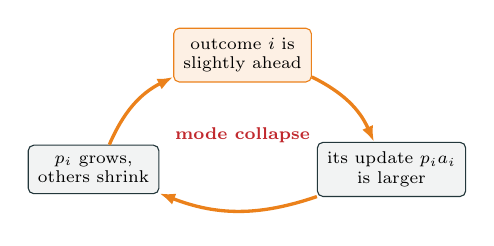
\begin{tikzpicture}[scale=0.88, transform shape]
  \node[ndh] (a) at (0,2.15)    {outcome $i$ is\\ slightly ahead};
  \node[nd]  (b) at (2.15,0.5)  {its update $p_i a_i$\\ is larger};
  \node[nd]  (c) at (-2.15,0.5) {$p_i$ grows,\\ others shrink};
  \draw[arh] (a) to[bend left=20] (b);
  \draw[arh] (b) to[bend left=20] (c);
  \draw[arh] (c) to[bend left=20] (a);
  \node[font=\scriptsize\bfseries, text=mRed] at (0,1.0) {mode collapse};
\end{tikzpicture}

\vspace{4mm}
{\scriptsize\raggedright
Collapse is a property of \alert{the objective itself}. Entropy bonuses and KL
penalties push against it, but they do not remove the cause.\par}
\end{column}
\end{columns}
\end{frame}

% --------------------------------------------------------------- 2
\begin{frame}{Base Paper: Inverse Probability Scaling}

\begin{columns}[T,onlytextwidth]
\begin{column}{0.53\textwidth}
\footnotesize
\textbf{Inverse Probability Scaling.} Divide the reward by the probability of the
outcome that produced it:
\[
  \tilde r(o) = \frac{r(o)}{p_\theta(o)} .
\]
The $1/p$ cancels the $p_i$ multiplier, so (Thm.~4.1, Cor.~4.2)
\[
  \dot z_i = r_i - p_i\!\sum_k r_k
  \;\;\Longrightarrow\;\;
  p_i^\star=\frac{r_i}{\sum_k r_k}.
\]

\medskip
In practice $p_\theta(o)$ is unknown. IPS-GRPO estimates it from a group of $G$
sampled rollouts and clips (their Eq.~9):
\[
  \tilde r(o_g)=\frac{r(o_g)}{\max\{\hat p(o_g),\,\varepsilon\}} .
\]
\end{column}

\begin{column}{0.45\textwidth}
\centering
\vspace{1mm}
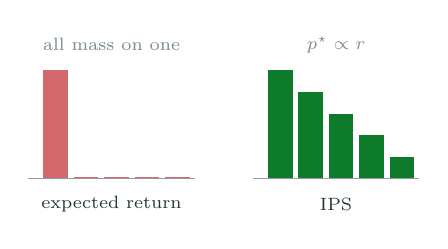
\begin{tikzpicture}[scale=0.92, transform shape]
  \def\bw{0.34}
  % left: collapse
  \begin{scope}
    \foreach \i/\h in {1/1.5,2/0.02,3/0.02,4/0.02,5/0.02}
      \fill[mRed!70] ({\i*0.42-0.21},0) rectangle ++(\bw,\h);
    \draw[mTeal!50] (0,0) -- (2.3,0);
    \node[font=\scriptsize, text=mTeal] at (1.15,-0.35) {expected return};
    \node[font=\scriptsize, text=mGrey] at (1.15,1.85) {all mass on one};
  \end{scope}
  % right: proportional
  \begin{scope}[xshift=3.1cm]
    \foreach \i/\h in {1/1.5,2/1.2,3/0.9,4/0.6,5/0.3}
      \fill[mGreen!70!black] ({\i*0.42-0.21},0) rectangle ++(\bw,\h);
    \draw[mTeal!50] (0,0) -- (2.3,0);
    \node[font=\scriptsize, text=mTeal] at (1.15,-0.35) {IPS};
    \node[font=\scriptsize, text=mGrey] at (1.15,1.85) {$p^\star\propto r$};
  \end{scope}
\end{tikzpicture}

\vspace{4mm}
{\scriptsize\raggedright
\textbf{Left open by the paper:}\par
\smallskip
1. Only two settings exist: plain (collapse) or exact proportionality.\par
\smallskip
2. The group size $G$ and clip $\varepsilon$ are ablated empirically only
(their Table 4).\par
\smallskip
3. Their own limitation section: finite-group estimates ``can be noisy,
requiring probability clipping that introduces a bias--variance trade-off''.
No analysis is given.\par}
\end{column}
\end{columns}
\end{frame}

% =====================================================================
\section{Project Overview}
% =====================================================================

% --------------------------------------------------------------- 3
\begin{frame}{Problem Statement and Extension}

\footnotesize
The paper gives one fixed correction. We asked three questions it does not answer.

\medskip
\begin{columns}[T,onlytextwidth]
\begin{column}{0.48\textwidth}
\textbf{1. Can the correction be tuned?}\par
Replace $r/p$ by $r/p^{\alpha}$. Redoing the paper's own gradient calculation gives
\[
  \dot z_i = r_i p_i^{1-\alpha}-p_i\!\sum_k r_k p_k^{1-\alpha},
  \qquad
  \boxed{\,p_i^\star \propto r_i^{1/\alpha}\,}
\]
One knob spans collapse, the paper's result, and near-uniform.

\medskip
\textbf{2. What does a finite group cost?}\par
Derive the effect of $G$ and $\varepsilon$ instead of ablating it.

\medskip
\textbf{3. How wrong is the estimate $\hat p$?}\par
The error analysis the paper lists as an open limitation.
\end{column}

\begin{column}{0.49\textwidth}
\centering
\vspace{-2mm}
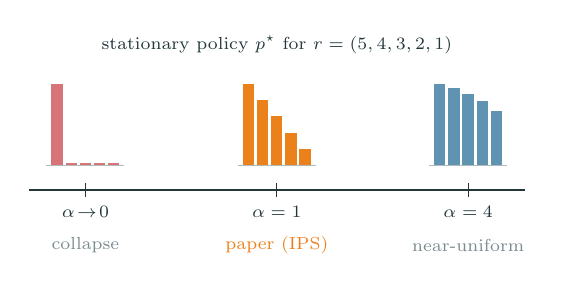
\begin{tikzpicture}[scale=0.9, transform shape]
  \node[font=\scriptsize, text=mTeal] at (3.7,2.05)
       {stationary policy $p^\star$ for $r=(5,4,3,2,1)$};
  % mini bar charts, each centred on its tick.  Group half-width = 0.48
  \def\bw{0.16}
  \foreach \xc/\col in {1.0/{mRed!65}, 3.7/{mOrange}, 6.4/{mBlue!75}}
    \draw[mTeal!35, thin] ({\xc-0.55},0.35) -- ({\xc+0.55},0.35);
  \begin{scope}[yshift=0.35cm]
    \foreach \i/\h in {1/1.15,2/0.03,3/0.03,4/0.03,5/0.03}
      \fill[mRed!65] ({1.0-0.48+(\i-1)*0.2},0) rectangle ++(\bw,\h);
    \foreach \i/\h in {1/1.15,2/0.92,3/0.69,4/0.46,5/0.23}
      \fill[mOrange] ({3.7-0.48+(\i-1)*0.2},0) rectangle ++(\bw,\h);
    \foreach \i/\h in {1/1.15,2/1.09,3/1.01,4/0.91,5/0.77}
      \fill[mBlue!75] ({6.4-0.48+(\i-1)*0.2},0) rectangle ++(\bw,\h);
  \end{scope}
  % axis
  \draw[thick, mTeal] (0.2,0) -- (7.2,0);
  \foreach \x/\l in {1.0/{$\alpha\!\to\!0$}, 3.7/{$\alpha=1$}, 6.4/{$\alpha=4$}}
    \draw[mTeal] (\x,0.1) -- (\x,-0.1) node[below, font=\scriptsize] {\l};
  \node[font=\scriptsize, text=mGrey]   at (1.0,-0.78) {collapse};
  \node[font=\scriptsize, text=mOrange] at (3.7,-0.78) {paper (IPS)};
  \node[font=\scriptsize, text=mGrey]   at (6.4,-0.78) {near-uniform};
\end{tikzpicture}

\vspace{3mm}
{\scriptsize\raggedright
$\alpha$ becomes a \alert{diversity dial}: the same algorithm, one extra
exponent.\par}
\end{column}
\end{columns}
\end{frame}

% --------------------------------------------------------------- 4
\begin{frame}{System Model}

\begin{columns}[T,onlytextwidth]
\begin{column}{0.46\textwidth}
\footnotesize
An \alert{outcome-selection bandit}: $K$ outcomes, fixed rewards $r_i>0$, policy
stored as logits and squashed by softmax,
\[
  p_i = \frac{e^{z_i}}{\sum_k e^{z_k}} .
\]

\medskip
Nothing else is in the model. No network, no exploration schedule, no critic. So
any collapse we see has \alert{exactly one possible cause}, which is the point the
paper argues.

\medskip
Two objects are studied throughout:
\begin{itemize}\setlength\itemsep{2pt}
  \item the \textbf{idealised flow} $\dot z=f(z)$, an ODE in $K$ variables;
  \item the \textbf{sampled update}, one noisy step built from $G$ draws.
\end{itemize}
\end{column}

\begin{column}{0.51\textwidth}
\centering
\vspace{1mm}
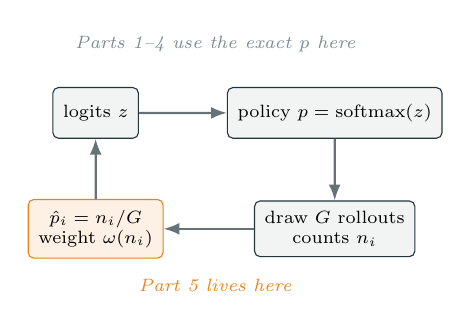
\begin{tikzpicture}[scale=0.92, transform shape]
  \node[nd]  (z)  at (0,1.6)   {logits $z$};
  \node[nd]  (p)  at (3.3,1.6) {policy $p=\mathrm{softmax}(z)$};
  \node[nd]  (s)  at (3.3,0)   {draw $G$ rollouts\\ counts $n_i$};
  \node[ndh] (ph) at (0,0)     {$\hat p_i = n_i/G$\\ weight $\omega(n_i)$};
  \draw[ar] (z) -- (p);
  \draw[ar] (p) -- (s);
  \draw[ar] (s) -- (ph);
  \draw[ar] (ph) -- (z);
  \node[lbl, align=center] at (1.65,2.55) {Parts 1--4 use the exact $p$ here};
  \node[lbl, align=center, text=mOrange] at (1.65,-0.78) {Part 5 lives here};
\end{tikzpicture}

\vspace{3mm}
{\scriptsize
\[
  \hat g_i=\hat p_i r_i\,\omega(n_i)-p_i\!\sum_k \hat p_k r_k\,\omega(n_k),
  \qquad z\leftarrow z+h\,\hat g
\]}
\end{column}
\end{columns}
\end{frame}

% --------------------------------------------------------------- 5
\begin{frame}{Work Breakdown}

\centering
\vspace{-1mm}
{\scriptsize
\begin{tabular}{@{}p{0.7cm} >{\raggedright\arraybackslash}p{3.8cm}
                            >{\raggedright\arraybackslash}p{7.9cm}@{}}
\toprule
\textbf{Part} & \textbf{Focus} & \textbf{Key content} \\
\midrule
1 & Collapse baseline, $\alpha=0$ &
  Integrate the flow with Euler and RK4, verify orders, show the exact tie is
  provably flat, and that sampling noise alone still collapses it \\
\addlinespace[2pt]
2 & The $\alpha$ knob &
  Stationary law $p^\star\!\propto r^{1/\alpha}$, linearisation and eigenvalue
  spectrum, convergence rates, explicit-method stability limits, first
  finite-$G$ ceiling \\
\addlinespace[2pt]
3 & Solving $\dot z = 0$ directly &
  Bisection, secant and Newton on three equivalent formulations; convergence
  orders, basins, conditioning; nested solver for the finite-$G$ fixed point \\
\addlinespace[2pt]
4 & Multi-parameter atlas &
  19{,}125 stationary points over $(\alpha,G,\varepsilon,\rho)$, support and
  entropy for general $K$, and whether interpolation can replace solving \\
\addlinespace[2pt]
5 & The estimator itself &
  Bias and variance of the clipped weight, Richardson extrapolation,
  golden-section search, power and QR methods, moving averages \\
\bottomrule
\end{tabular}}

\vspace{4mm}
{\footnotesize
One shared library (\texttt{src/}), one script per part
(\texttt{experiments/}), one write-up per part, and 68 unit tests.}
\end{frame}

% =====================================================================
\section{Part 1: Collapse Baseline}
% =====================================================================

% --------------------------------------------------------------- P1.1
\begin{frame}{Part 1: Objective}

\begin{columns}[T,onlytextwidth]
\begin{column}{0.45\textwidth}
\footnotesize
Before correcting collapse we had to reproduce it, and to be precise about a claim
the paper states informally.

\medskip
The paper says collapse happens ``even with exactly equal rewards''. For the
\alert{deterministic} flow that is not literally true: if all $r_i$ are equal then
$a_i\equiv 0$, so $\dot z\equiv 0$ and nothing moves at all.

\medskip
What actually drives collapse under a tie is \alert{sampling noise}. A finite group
never sees the exact mean reward, so the realised advantage is never zero, and the
$p_i$ multiplier then amplifies it.

\medskip
So Part 1 runs both and separates them.
\end{column}

\begin{column}{0.52\textwidth}
\centering
\vspace{-4mm}
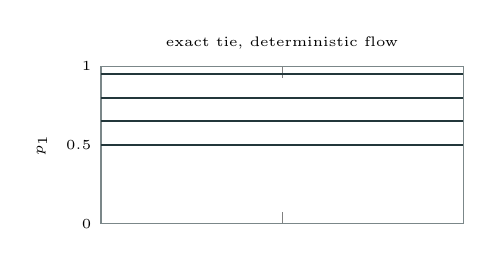
\begin{tikzpicture}
\begin{axis}[
  width=4.6cm, height=2.0cm, scale only axis,
  ylabel={$p_1$},
  xmin=0, xmax=300, ymin=0, ymax=1,
  xtick={0,150,300}, xticklabels={,,}, ytick={0,0.5,1},
  label style={font=\tiny}, tick label style={font=\tiny},
  title={\tiny exact tie, deterministic flow}, title style={yshift=-1.2mm},
  axis line style={mTeal!60}, every axis plot/.append style={thick},
]
  \addplot[mTeal, domain=0:300]{0.50};
  \addplot[mTeal, domain=0:300]{0.65};
  \addplot[mTeal, domain=0:300]{0.80};
  \addplot[mTeal, domain=0:300]{0.95};
\end{axis}
\end{tikzpicture}

\vspace{1mm}
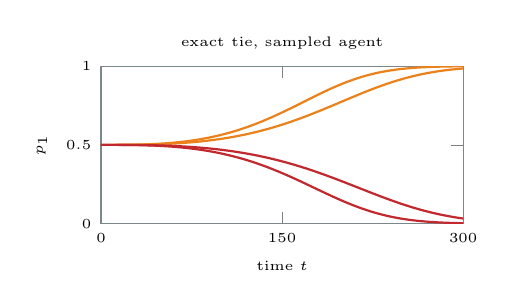
\begin{tikzpicture}
\begin{axis}[
  width=4.6cm, height=2.0cm, scale only axis,
  xlabel={time $t$}, ylabel={$p_1$},
  xmin=0, xmax=300, ymin=0, ymax=1,
  xtick={0,150,300}, ytick={0,0.5,1},
  label style={font=\tiny}, tick label style={font=\tiny},
  title={\tiny exact tie, sampled agent}, title style={yshift=-1.2mm},
  axis line style={mTeal!60}, every axis plot/.append style={thick},
]
  % all four start at exactly 0.5 and drift apart, as in Exp. 1 Fig. 2a
  \addplot[mOrange, domain=0:300, samples=120]{1/(1+exp(-7.0*(x/300)^3))};
  \addplot[mOrange, domain=0:300, samples=120]{1/(1+exp(-4.2*(x/300)^3))};
  \addplot[mRed,    domain=0:300, samples=120]{1/(1+exp( 6.0*(x/300)^3))};
  \addplot[mRed,    domain=0:300, samples=120]{1/(1+exp( 3.4*(x/300)^3))};
\end{axis}
\end{tikzpicture}

\vspace{2mm}
{\scriptsize Same rewards, same starting policy. Only the noise differs.}
\end{column}
\end{columns}
\end{frame}

% --------------------------------------------------------------- P1.2
\begin{frame}{Part 1: Numerical Methods}

\footnotesize
\begin{columns}[T,onlytextwidth]
\begin{column}{0.48\textwidth}

\textbf{Solution of ODEs.}
The flow is a coupled system in $K$ unknowns,
\[
  \dot z_i = r_i p_i - p_i\!\sum_k r_k p_k .
\]
Integrated with Euler
$z_{n+1}=z_n+h f(z_n)$
and classical RK4
\[
  z_{n+1}=z_n+\tfrac{h}{6}(k_1+2k_2+2k_3+k_4).
\]

\medskip
\textbf{Truncation and round-off error.}
Empirical order from a step-size sweep,
\[
  \text{order}=\text{slope of }\log E \text{ vs }\log h .
\]
Below $h\approx 0.025$ the RK4 error stops falling: the truncation term has
dropped under the round-off floor.

\end{column}
\begin{column}{0.48\textwidth}

\textbf{Least-squares regression.}
Collapse time against reward gap, fitted in log-log space,
\[
  \log t_{\text{col}} = m\log\Delta + c
  \;\Rightarrow\; t_{\text{col}}\approx 53.94\,\Delta^{-1.00}.
\]
The same fit gives the group-size law $t_{\text{col}}\propto G^{1.07}$.

\medskip
\textbf{Random number generation.}
The sampled agent draws outcomes by \alert{inverse transform sampling}: build the
CDF of $p$, draw $u\sim U(0,1)$, take
\[
  o=\min\{\,i : \textstyle\sum_{k\le i}p_k \ge u\,\}.
\]

\medskip
\textbf{Visualisation.} Semi-log and log-log axes, since both the transition and
the fitted laws span decades.

\end{column}
\end{columns}
\end{frame}

% --------------------------------------------------------------- P1.3
\begin{frame}{Part 1: Results and Analysis}

\footnotesize
\begin{columns}[T,onlytextwidth]
\begin{column}{0.5\textwidth}
\textbf{The tie is provably flat.} Four different starting policies, $T=300$:
\[
  \max_t |\Delta p_1| = \hit{$1.11\times10^{-16}$}
\]
which is machine epsilon, not a slow drift. This \alert{sharpens} the paper's claim
rather than contradicting it.

\medskip
\textbf{Noise alone collapses it.} From an exactly symmetric start ($z_0=0$),
$K=5$, 200 seeds:

\centering
{\scriptsize
\begin{tabular}{@{}lccccc@{}}
\toprule
outcome & O1 & O2 & O3 & O4 & O5 \\
\midrule
won & 18.5\% & 22.5\% & 19.0\% & 19.0\% & 21.0\% \\
\bottomrule
\end{tabular}}

\raggedright\smallskip
All inside the 95\% band $[14.5,25.5]\%$ around $1/K$. The winner is arbitrary.
\end{column}

\begin{column}{0.47\textwidth}
\textbf{Two clean scaling laws.}
\[
  t_{\text{col}}\approx 53.94\,\Delta^{-1.00},\quad R^2=0.99999994
\]
\[
  t_{\text{col}}\propto G^{1.07},\quad R^2=0.974
\]
A bigger group delays collapse roughly linearly. That is a statement about a real
GRPO hyperparameter.

\medskip
\textbf{Integrators behave.}

\centering
{\scriptsize
\begin{tabular}{@{}lcc@{}}
\toprule
 & order & error at $h=0.05$ \\
\midrule
Euler & 1.00 & $1.4\times10^{-4}$ \\
RK4   & 3.99 & $5.1\times10^{-8}$ \\
\bottomrule
\end{tabular}}

\raggedright\smallskip
\medskip
\textbf{Reported honestly:} we looked for an Euler instability here and found
none. The right-hand side is bounded and self-damping at $\alpha=0$, so no step
size can overshoot. Part 2 is where instability appears.
\end{column}
\end{columns}
\end{frame}

% =====================================================================
\section{Part 2: The Diversity Exponent}
% =====================================================================

% --------------------------------------------------------------- P2.1
\begin{frame}{Part 2: Objective}

\begin{columns}[T,onlytextwidth]
\begin{column}{0.48\textwidth}
\footnotesize
Test every prediction of the $\alpha$ generalisation, first on the exact ODE and
then on the sampled agent.

\medskip
\begin{itemize}\setlength\itemsep{3pt}
  \item Does the flow really settle at $p^\star\propto r^{1/\alpha}$?
  \item \emph{How fast} does it get there, and can we predict the rate before
        running anything?
  \item Which step sizes are safe for an explicit method?
  \item Does a finite group change the answer?
\end{itemize}

\medskip
The last question produced the result that the rest of the project is built on.
\end{column}

\begin{column}{0.49\textwidth}
\centering
\vspace{-4mm}
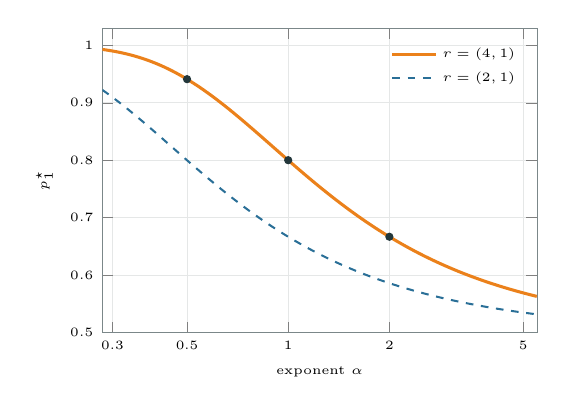
\begin{tikzpicture}[scale=0.92, transform shape]
\begin{axis}[
  width=6.0cm, height=4.2cm, scale only axis,
  xlabel={exponent $\alpha$}, ylabel={$p_1^\star$},
  xmode=log, xmin=0.28, xmax=5.5, ymin=0.5, ymax=1.03,
  xtick={0.3,0.5,1,2,5}, xticklabels={0.3,0.5,1,2,5},
  ytick={0.5,0.6,0.7,0.8,0.9,1.0},
  label style={font=\tiny}, tick label style={font=\tiny},
  axis line style={mTeal!60}, grid=major, grid style={mTeal!12},
  legend style={font=\tiny, draw=none, fill=none, at={(0.98,0.97)}, anchor=north east},
]
  \addplot[mOrange, very thick, domain=0.28:5.5, samples=120]
    {(4^(1/x))/((4^(1/x))+1)};
  \addlegendentry{$r=(4,1)$}
  \addplot[mBlue, thick, dashed, domain=0.28:5.5, samples=120]
    {(2^(1/x))/((2^(1/x))+1)};
  \addlegendentry{$r=(2,1)$}
  \addplot[only marks, mark=*, mark size=1.4pt, mTeal]
    coordinates {(0.5,0.941176) (1,0.8) (2,0.666667)};
\end{axis}
\end{tikzpicture}

\vspace{1mm}
{\scriptsize\raggedright
Marked points: $94/6$, $80/20$, $67/33$. RK4 endpoints land on the analytic
curve to $7.5\times10^{-15}$.\par}
\end{column}
\end{columns}
\end{frame}

% --------------------------------------------------------------- P2.2
\begin{frame}{Part 2: Numerical Methods (1/2)}

\footnotesize
\begin{columns}[T,onlytextwidth]
\begin{column}{0.49\textwidth}

\textbf{Modelling with differential equations.}
Stationary points come from setting $\dot z_i=0$, so $r_i p_i^{-\alpha}$ must be the
same constant for every $i$:
\[
  p_i^\star \propto r_i^{1/\alpha}.
\]

\medskip
\textbf{Eigenvalue decomposition.}
Linearise at $p^\star$. With the softmax derivative
$C=\mathrm{diag}(p^\star)-p^\star p^{\star\top}$, perturbing the flow gives
\[
  J^\star=-\alpha\lVert r\rVert_{1/\alpha}\,C .
\]
$J^\star$ is symmetric negative semidefinite. Its nonzero eigenvalues are the
convergence rates
\[
  \lambda_j=\alpha\lVert r\rVert_{1/\alpha}\,\mu_j ,
\]
with $\mu_j$ the nonzero eigenvalues of $C$. One zero eigenvalue survives, along
$\mathbf 1$, because shifting all logits leaves $p$ unchanged.

\end{column}
\begin{column}{0.47\textwidth}

\textbf{Least-squares regression.}
Fit $\ln\lVert p(t)-p^\star\rVert_1$ against $t$ inside a window past the
nonlinear transient and above round-off. The slope is the measured rate, checked
against $\lambda_{\min}$ above.

\medskip
\textbf{Round-off error.}
The fit window is chosen as $[10^{-12},10^{-6}]$ precisely because below
$10^{-12}$ the error is round-off, not dynamics.

\medskip
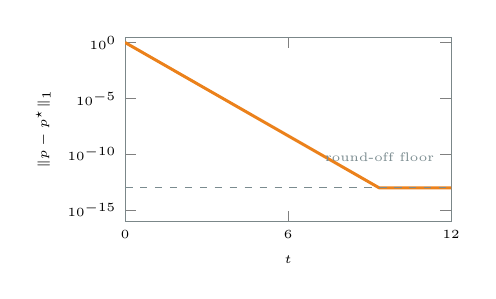
\begin{tikzpicture}[scale=0.9, transform shape]
\begin{axis}[
  width=4.6cm, height=2.6cm, scale only axis,
  xlabel={$t$}, ylabel={$\lVert p-p^\star\rVert_1$},
  ymode=log, xmin=0, xmax=12, ymin=1e-16, ymax=3,
  ytick={1e-15,1e-10,1e-5,1}, xtick={0,6,12},
  label style={font=\tiny}, tick label style={font=\tiny},
  axis line style={mTeal!60},
]
  \addplot[mOrange, very thick, domain=0:12, samples=200]
    {max(exp(-3.2*x), 1e-13)};
  \addplot[mGrey, dashed, domain=0:12, samples=2]{1e-13};
  \node[font=\tiny, text=mGrey, anchor=south east]
    at (axis cs:11.7,4e-12) {round-off floor};
\end{axis}
\end{tikzpicture}

\end{column}
\end{columns}
\end{frame}

% --------------------------------------------------------------- P2.3
\begin{frame}{Part 2: Numerical Methods (2/2)}

\footnotesize
\begin{columns}[T,onlytextwidth]
\begin{column}{0.5\textwidth}

\textbf{Stability of explicit ODE methods.}
A linear mode with rate $\lambda$ is stable only if
\[
  h\lambda_{\max} < 2 \;\;(\text{Euler}),
  \qquad
  h\lambda_{\max} < 2.7853\;\;(\text{RK4}).
\]
The RK4 constant is the real root of
$x^3-4x^2+12x-24=0$, which we obtain by \alert{bisection} rather than quoting it.

\medskip
\textbf{Root finding: bisection.}
The critical step size is found by bisection \emph{on the actual nonlinear
iteration}: shrink or grow $h$ until a $10^{-4}$ perturbation of $z^\star$ stops
decaying. It matches the linear theory to $2.6\times10^{-4}$ (Euler) and
$1.3\times10^{-4}$ (RK4).

\end{column}
\begin{column}{0.46\textwidth}

\textbf{Random number generation and simulation.}
The sampled agent is one noisy Euler step per iteration. Group frequencies obey
\[
  G\hat p_i \sim \mathrm{Binomial}(G,p_i).
\]
Taking the expectation of that update replaces $p_i^{-\alpha}$ by an
\alert{effective weight}
\[
  w_G(p)=\frac{\mathbb{E}\!\left[\hat p\,\omega(n)\right]}{p},
\]
whose stationary condition $r_i w_G(p_i)=S$ is solved by bisection.

\medskip
\textbf{Model validation.} Every Monte-Carlo run is compared against that
mean-field prediction, which is the $h\to0$ limit of the same update.

\end{column}
\end{columns}
\end{frame}

% --------------------------------------------------------------- P2.4
\begin{frame}{Part 2: Results and Analysis}

\footnotesize
\begin{columns}[T,onlytextwidth]
\begin{column}{0.49\textwidth}
\textbf{The knob works, and the rate is predictable.}
Fitted rate against $\lambda_{\min}$ from the Jacobian: relative error
$\le \hit{$1.7\times10^{-5}$}$ over 27 runs ($K=2$).

\medskip
\textbf{Both ends of the dial are numerically hard.}

\centering
{\scriptsize
\begin{tabular}{@{}lccc@{}}
\toprule
$\alpha$ & $\lambda_{\min}$ & $\lambda_{\max}$ & ratio \\
\midrule
0.1 & $5.8\times10^{-8}$ & 0.089 & $1.5\times10^{6}$ \\
1   & 1.15 & 4.53 & 3.9 \\
5   & $7.2\times10^{3}$ & $9.3\times10^{3}$ & 1.3 \\
\bottomrule
\end{tabular}}

\raggedright\smallskip
\medskip
Small $\alpha$ is stiff (huge spread of time scales). Large $\alpha$ makes every
rate large, so stability, not accuracy, sets $h$. Part 1's step $h=0.05$ becomes
unstable above $\alpha=2.06$ for Euler.

\medskip
$\alpha=0$ is a \alert{singular limit}: the approach is algebraic,
$p_2\sim 1/(2\Delta t)$, fitted tail slope $-1.007$, with no exponential rate at all.
\end{column}

\begin{column}{0.48\textwidth}
\textbf{The result the project is built on.}
A group of $G$ sees a rare outcome at most once, at frequency $1/G$. So the
inverse-probability weight is \alert{capped}:
\[
  w_G(p)\;\longrightarrow\;\min\{G,1/\varepsilon\}^{\alpha}
  \quad\text{as } p\to 0 .
\]
The minority outcome survives only if
\[
  \boxed{\;\alpha > \alpha_c=\frac{\ln(r_1/r_2)}{\ln\min\{G,1/\varepsilon\}}\;}
\]

\centering
{\scriptsize
\begin{tabular}{@{}lccccc@{}}
\toprule
$G$ & 4 & 8 & 16 & 32 & 64 \\
\midrule
$\alpha_c$, $r=(4,1)$ & 1.0 & 0.667 & 0.5 & 0.4 & 0.333 \\
\bottomrule
\end{tabular}}

\raggedright\smallskip
\medskip
\bad{At $G=4$ the paper's own $\alpha=1$ fails}: long-run $p_1=0.9965$ instead of
$0.8$. Monte Carlo tracks the mean field to $0.013$ worst case.
\end{column}
\end{columns}
\end{frame}

% =====================================================================
\section{Part 3: Root Finding Methods}
% =====================================================================

% --------------------------------------------------------------- P3.1
\begin{frame}{Part 3: Objective}

\begin{columns}[T,onlytextwidth]
\begin{column}{0.47\textwidth}
\footnotesize
Part 2 reached $p^\star$ by integrating for many e-folding times. Part 3 solves
$\dot z=0$ \alert{directly} and checks the root against the analytic answer.

\medskip
The same condition can be written three ways:
\[
\begin{aligned}
\text{drift:}   &\quad F_i=\dot z_i \\
\text{balance:} &\quad F_i=r_ip_i^{-\alpha}-r_Kp_K^{-\alpha} \\
\text{log:}     &\quad F_i=\ln\tfrac{r_i}{r_K}-\alpha(z_i-z_K)
\end{aligned}
\]

\medskip
They share the same root. Dividing by $p_i$ removes the very multiplier the paper
blames for collapse, and it turns out to matter for Newton too.
\end{column}

\begin{column}{0.5\textwidth}
\centering
\vspace{-4mm}
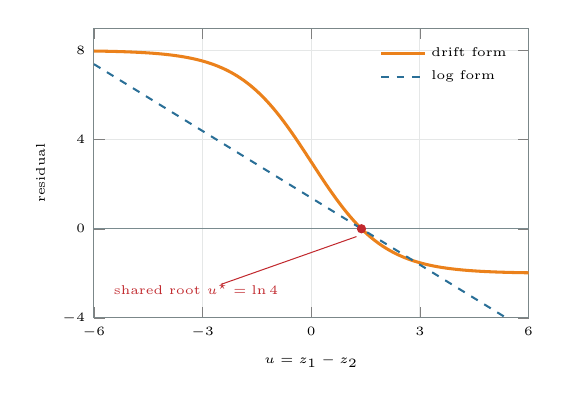
\begin{tikzpicture}[scale=0.92, transform shape]
\begin{axis}[
  width=6.0cm, height=4.0cm, scale only axis,
  xlabel={$u=z_1-z_2$}, ylabel={residual},
  xmin=-6, xmax=6, ymin=-4, ymax=9,
  xtick={-6,-3,0,3,6}, ytick={-4,0,4,8},
  label style={font=\tiny}, tick label style={font=\tiny},
  axis line style={mTeal!60}, grid=major, grid style={mTeal!12},
  legend style={font=\tiny, draw=none, fill=none, at={(0.98,0.97)},
                anchor=north east, legend cell align=left},
]
  % drift for r=(4,1), alpha=1:  g(u) = 8 - 10*sigmoid(u)
  \addplot[mOrange, very thick, domain=-6:6, samples=120]{8-10/(1+exp(-x))};
  \addlegendentry{drift form}
  % log form: ln4 - u
  \addplot[mBlue, thick, dashed, domain=-6:6, samples=2]{1.3863-x};
  \addlegendentry{log form}
  \addplot[mGrey, domain=-6:6, samples=2]{0};
  \addplot[only marks, mark=*, mark size=1.6pt, mRed] coordinates {(1.3863,0)};
  \node[font=\tiny, text=mRed, anchor=west] at (axis cs:-5.7,-2.7)
    {shared root $u^\star=\ln 4$};
  \draw[mRed, thin] (axis cs:-2.5,-2.5) -- (axis cs:1.25,-0.35);
\end{axis}
\end{tikzpicture}

\vspace{0mm}
{\scriptsize\raggedright
The drift saturates at both ends, so a Newton step taken from far out lands even
further away. The log form is a straight line, so Newton solves it in one
step.\par}
\end{column}
\end{columns}
\end{frame}

% --------------------------------------------------------------- P3.2
\begin{frame}{Part 3: Numerical Methods}

\footnotesize
\begin{columns}[T,onlytextwidth]
\begin{column}{0.48\textwidth}

\textbf{Root finding.} All three from the syllabus, on the same problem:
\[
\begin{aligned}
\text{bisection:} &\quad \text{halve a sign-change bracket} \\
\text{secant:}    &\quad u_{n+1}=u_n-F_n\tfrac{u_n-u_{n-1}}{F_n-F_{n-1}} \\
\text{Newton:}    &\quad u_{n+1}=u_n-F(u_n)/F'(u_n)
\end{aligned}
\]
Measured order from the least-squares slope of $\ln e_{n+1}$ against $\ln e_n$.

\medskip
\textbf{Systems of equations.} For $K>2$, Newton solves
\[
  J(y)\,\delta y=-F(y)
\]
by Gaussian elimination each iteration. $J$ is the analytic Jacobian, not a
finite difference.

\end{column}
\begin{column}{0.48\textwidth}

\textbf{Conditioning, and a gauge.}
Shifting every logit leaves $\dot z$ unchanged, so $J\mathbf 1=0$ and the full
$K\times K$ system is \alert{singular} (smallest singular value
$7.1\times10^{-17}$). Fixing $z_K=0$ removes it. At the root
\[
  J_{\text{balance}}=-\alpha\lVert r\rVert_{1/\alpha}I,
  \qquad
  J_{\text{log}}=-\alpha I,
\]
so both have condition number exactly 1.

\medskip
\textbf{Nested root finding for finite $G$.}
Inner: invert the monotone $w_G(p_i)=S/r_i$ for each outcome.
Outer: choose $S$ with $\sum_i p_i(S)=1$. Both levels are monotone with a
guaranteed bracket, so bisection is safe and safeguarded Newton is fast.

\end{column}
\end{columns}
\end{frame}

% --------------------------------------------------------------- P3.3
\begin{frame}{Part 3: Results and Analysis}

\footnotesize
\begin{columns}[T,onlytextwidth]
\begin{column}{0.46\textwidth}
\textbf{Textbook orders, confirmed.} $K=2$, $\alpha=1$, root $u^\star=\ln4$:

\centering
{\scriptsize
\begin{tabular}{@{}lcc@{}}
\toprule
method & iterations & order \\
\midrule
bisection & 56 & linear (0.502) \\
secant    &  9 & \hit{1.61} \\
Newton (drift)   & 5 & \hit{2.00} \\
Newton (log)     & 1 & exact \\
\bottomrule
\end{tabular}}

\raggedright\smallskip
\medskip
\textbf{How you write the equation decides the basin.}
Newton on the drift form converges from only \bad{17\%} of starts at $\alpha=1$,
but from 100\% once $\alpha>1.113$. On the balance form it converges from
\good{100\%} of starts at every $\alpha$.

\medskip
Backtracking does not rescue it: for $\alpha<1$ every simplex vertex is a zero of
the drift ``at infinity'', and a line search is pulled into them.
\end{column}

\begin{column}{0.5\textwidth}
\textbf{Nested solver: Newton pays off.} Over $G\in\{4,16,64\}\times\alpha\in\{0.5,1,2\}$:

\centering
{\scriptsize
\begin{tabular}{@{}lcc@{}}
\toprule
 & outer iters & total work \\
\midrule
bisection / bisection & 43--55 & 4{,}506--13{,}769 \\
Newton / Newton       & 6--16  & \hit{225--1{,}703} \\
\bottomrule
\end{tabular}}

\raggedright\smallskip
Same answer to $9.8\times10^{-14}$, with 8 to 20 times less work.

\medskip
\textbf{A new result for $K>2$.} The two-outcome threshold understates the
requirement. At $G=16$, $r=(5,4,3,2,1)$:

\centering
{\scriptsize
\begin{tabular}{@{}lcccc@{}}
\toprule
$\alpha_c$ for & O2 & O3 & O4 & O5 \\
\midrule
$K=5$ mean field & 0.0805 & 0.203 & 0.419 & \hit{0.886} \\
pairwise formula & 0.0805 & 0.184 & 0.330 & 0.580 \\
\bottomrule
\end{tabular}}

\raggedright
\smallskip
Some outcomes are lost at \alert{every} $\alpha$: here the weakest needs
$G\ge6$ before any exponent can keep it.
\end{column}
\end{columns}
\end{frame}

% =====================================================================
\section{Part 4: Parameter Atlas}
% =====================================================================

% --------------------------------------------------------------- P4.1
\begin{frame}{Part 4: Objective}

\begin{columns}[T,onlytextwidth]
\begin{column}{0.46\textwidth}
\footnotesize
Parts 2 and 3 varied one or two parameters. Part 4 asks whether the survival
boundary really holds \alert{jointly} over all four, and whether a grid can stand
in for solving.

\medskip
The predicted boundary collapses to a single signed margin
\[
  m=\alpha\log\min\{G,\tfrac1\varepsilon\}-\log\rho ,
\]
with $\rho=r_1/r_2$. Survival should be exactly $m>0$, independent of where in the
four-dimensional box you are.

\medskip
$19{,}125$ stationary points were solved to test that one inequality.
\end{column}

\begin{column}{0.51\textwidth}
\centering
\vspace{-4mm}
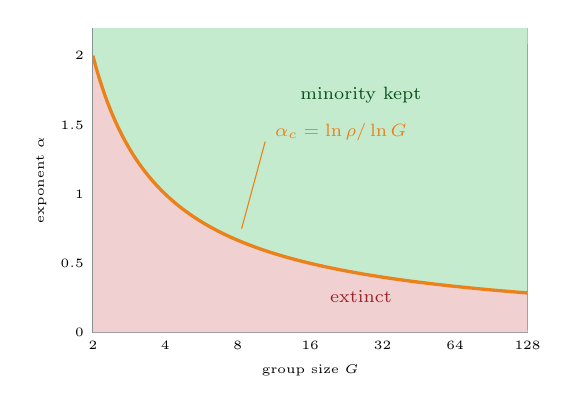
\begin{tikzpicture}[scale=0.92, transform shape]
\begin{axis}[
  width=6.0cm, height=4.2cm, scale only axis,
  xlabel={group size $G$}, ylabel={exponent $\alpha$},
  xmode=log, log basis x=2, xmin=2, xmax=128, ymin=0, ymax=2.2,
  xtick={2,4,8,16,32,64,128}, xticklabels={2,4,8,16,32,64,128},
  ytick={0,0.5,1,1.5,2},
  label style={font=\tiny}, tick label style={font=\tiny},
  axis line style={mTeal!60},
]
  \addplot[name path=curve, mOrange, very thick, domain=2:128, samples=120]
    {ln(4)/ln(x)};
  \path[name path=top] (axis cs:2,2.2) -- (axis cs:128,2.2);
  \path[name path=bot] (axis cs:2,0)   -- (axis cs:128,0);
  \addplot[mGreen!25] fill between[of=curve and top];
  \addplot[mRed!22]   fill between[of=curve and bot];
  \node[font=\scriptsize, text=mGreen!45!black] at (axis cs:26,1.72) {minority kept};
  \node[font=\scriptsize, text=mRed!80!black]   at (axis cs:26,0.26) {extinct};
  \node[font=\scriptsize, text=mOrange, anchor=west] at (axis cs:10.5,1.45)
    {$\alpha_c=\ln\rho/\ln G$};
  \draw[mOrange, thin] (axis cs:10.4,1.38) -- (axis cs:8.3,0.75);
\end{axis}
\end{tikzpicture}

\vspace{0mm}
{\scriptsize One slice ($\rho=4$, $\varepsilon=10^{-3}$) of a four-dimensional atlas.}
\end{column}
\end{columns}
\end{frame}

% --------------------------------------------------------------- P4.2
\begin{frame}{Part 4: Numerical Methods}

\footnotesize
\begin{columns}[T,onlytextwidth]
\begin{column}{0.48\textwidth}

\textbf{Interpolation.}
The atlas is a tensor-product grid in $(\log\alpha,\log\rho,\log\varepsilon)$.
Inside one cell, with $t_d\in[0,1]$ the fractional position along axis $d$, the
\alert{multilinear} interpolant is the weighted sum over the cell's $2^D$ corners:
\[
  \hat f(\mathbf x)=\sum_{\mathbf c\in\{0,1\}^D}
      f(\mathbf x_{\mathbf c})\prod_{d=1}^{D}t_d^{c_d}(1-t_d)^{1-c_d}.
\]
This is the $D$-dimensional form of the linear interpolation in the syllabus, and
it is exact at nodes and for any function affine in each coordinate separately.

\medskip
\textbf{Approximation error and order.}
Refine the grid and fit the slope of $\log(\text{RMSE})$ against
$\log(\text{intervals per axis})$.

\end{column}
\begin{column}{0.48\textwidth}

\textbf{Root finding, vectorised.}
All $19{,}125$ $K=2$ solves run as one batched bisection with 64 deterministic
halvings, and 40 of them are re-checked against the original scalar solver.

\medskip
\textbf{Model validation and verification.}
The script refuses to write a summary unless every check passes:
phase classification, stationarity residual, normalisation, node exactness, and
monotone refinement.

\medskip
\textbf{Where the theory says interpolation must degrade.}
The response is continuous but has derivative kinks at
\[
  m=0 \;\;(\text{extinction}),
  \qquad
  \varepsilon=1/G \;\;(\text{clip activates}),
\]
so cells crossing those surfaces cannot keep second-order behaviour. We measure
the two regions separately instead of quoting one rate.

\end{column}
\end{columns}
\end{frame}

% --------------------------------------------------------------- P4.3
\begin{frame}{Part 4: Results and Analysis}

\footnotesize
\begin{columns}[T,onlytextwidth]
\begin{column}{0.47\textwidth}
\textbf{The boundary holds everywhere.}
Over $51\times15\times5\times5=19{,}125$ points:
\[
  \text{misclassifications} = \hit{$0/19{,}125$}
\]
with worst stationarity residual $1.18\times10^{-15}$.

\medskip
\textbf{Two separate ceilings.} $\varepsilon$ can bind before $G$ does. At
$\alpha=1$, $\rho=4$:

\centering
{\scriptsize
\begin{tabular}{@{}lcccc@{}}
\toprule
$p_2$ at & $G{=}6$ & $G{=}16$ & $G{=}64$ & $G{=}256$ \\
\midrule
$\varepsilon=10^{-3}$ & 0.115 & 0.195 & 0.200 & 0.200 \\
$\varepsilon=0.3$     & 0 & 0 & 0 & \bad{0} \\
\bottomrule
\end{tabular}}

\raggedright\smallskip
With $\varepsilon=0.3$ the clip caps the boost at $3.33<4$, so \alert{no group size
whatsoever} rescues the minority.
\end{column}

\begin{column}{0.49\textwidth}
\textbf{Group size must grow with the problem.}
Smallest $G$ that keeps every outcome at $\alpha=1$:

\centering
{\scriptsize
\begin{tabular}{@{}lcc@{}}
\toprule
$K$ & spread 1.25 & spread 32 \\
\midrule
2  & 2 & 33 \\
5  & 3 & 54 \\
10 & 4 & \hit{96} \\
\bottomrule
\end{tabular}}

\raggedright\smallskip
A best-versus-worst ratio alone does not predict this once several strong
outcomes compete for mass.

\medskip
\textbf{Interpolation audit.} 800 held-out off-grid points:

\centering
{\scriptsize
\begin{tabular}{@{}lcc@{}}
\toprule
region & RMSE ($17^3$) & order \\
\midrule
smooth        & $2.5\times10^{-3}$ & \good{1.58} \\
near a kink   & $9.7\times10^{-3}$ & \bad{1.03} \\
\bottomrule
\end{tabular}}

\raggedright
\smallskip
So a grid is fine for exploring, but survival decisions near $m=0$ need a real
solve. The margin $m$ is useful twice: as the criterion, and as a warning flag.
\end{column}
\end{columns}
\end{frame}

% =====================================================================
\section{Part 5: Estimator Error Analysis}
% =====================================================================

% --------------------------------------------------------------- P5.1
\begin{frame}{Part 5: Objective}

\begin{columns}[T,onlytextwidth]
\begin{column}{0.44\textwidth}
\footnotesize
Parts 1 to 4 assume the update knows $p$. It does not. It has $G$ samples, and it
needs $p^{-\alpha}$.

\medskip
This is the paper's own stated limitation, and it is a pure
\alert{error-analysis} problem: bias against variance, with a knob ($\varepsilon$)
that trades one for the other exactly like a step size trades truncation against
round-off.

\medskip
We compare the paper's clipped rule against three alternatives, and ask which
trade the \emph{learning dynamics} actually notice.
\end{column}

\begin{column}{0.53\textwidth}
\centering
\vspace{-2mm}
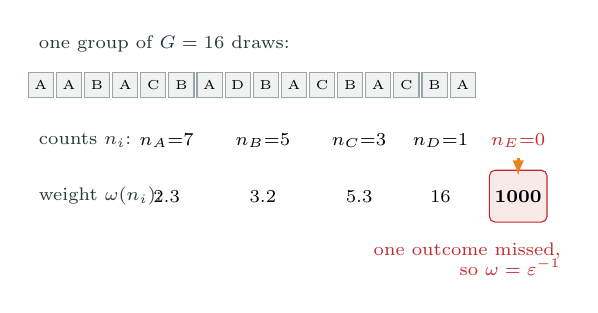
\begin{tikzpicture}[scale=0.94, transform shape]
  \node[font=\scriptsize, text=mTeal, anchor=west] at (0,2.75)
       {one group of $G=16$ draws:};
  % the draws
  \foreach \i/\c in {0/A,1/A,2/B,3/A,4/C,5/B,6/A,7/D,8/B,9/A,10/C,11/B,12/A,13/C,14/B,15/A}{
    \node[draw=mTeal!45, fill=mTeal!7, minimum size=3.4mm, inner sep=0pt,
          font=\tiny] at ({0.15+\i*0.38},2.2) {\c};
  }
  % counts row
  \node[font=\scriptsize, text=mTeal, anchor=west] at (0,1.45) {counts $n_i$:};
  \foreach \x/\t in {1.85/{$n_A{=}7$}, 3.15/{$n_B{=}5$}, 4.45/{$n_C{=}3$},
                     5.55/{$n_D{=}1$}}
    \node[font=\scriptsize] at (\x,1.45) {\t};
  \node[font=\scriptsize, text=mRed] at (6.6,1.45) {$n_E{=}0$};
  % weights row
  \node[font=\scriptsize, text=mTeal, anchor=west] at (0,0.7)
       {weight $\omega(n_i)$:};
  \foreach \x/\t in {1.85/{2.3}, 3.15/{3.2}, 4.45/{5.3}, 5.55/{16}}
    \node[font=\scriptsize] at (\x,0.7) {\t};
  \node[ndr, inner sep=2pt] at (6.6,0.7) {\textbf{1000}};
  \draw[arh] (6.6,1.22) -- (6.6,0.97);
  \node[font=\scriptsize, text=mRed, align=right, anchor=north east] at (7.3,0.2)
    {one outcome missed,\\ so $\omega=\varepsilon^{-1}$};
\end{tikzpicture}

\vspace{1mm}
{\scriptsize\raggedright
Without the clip that entry is $\infty$. With it, one unlucky group hands a rare
outcome a weight 60 times larger than anything else in the same group.\par}
\end{column}
\end{columns}
\end{frame}

% --------------------------------------------------------------- P5.2
\begin{frame}{Part 5: Numerical Methods (1/2)}

\footnotesize
\begin{columns}[T,onlytextwidth]
\begin{column}{0.49\textwidth}

\textbf{Truncation error via Taylor expansion.}
Expand $f(x)=x^{-\alpha}$ about $p$ with the random step $\hat p-p$, take
expectations, and use the binomial central moments
($\mathbb{E}[\hat p]=p$, $\mathrm{Var}=pq/G$):
\[
  \mathbb{E}[f(\hat p)]=f(p)+\tfrac12 f''(p)\tfrac{pq}{G}+O(G^{-2}),
\]
which gives the relative bias and standard deviation
\[
  b=\frac{\alpha(\alpha+1)(1-p)}{2Gp},
  \qquad
  s=\alpha\sqrt{\frac{1-p}{Gp}} .
\]
The small parameter is \alert{$Gp$}, the expected number of hits, not $G$.

\end{column}
\begin{column}{0.47\textwidth}

\textbf{Golden-section search.}
$\mathrm{MSE}(\varepsilon)$ falls then rises, with kinks at every
$\varepsilon=n/G$, so a derivative-free bracketing minimiser is the right tool.
It shrinks the bracket by $1/\phi=0.618$ per evaluation.

\medskip
\textbf{Richardson extrapolation.}
Equation above is an expansion in $1/G$ with $G$-independent coefficients, so the
standard combination applies. Splitting the group into halves of size $M=G/2$:
\[
  \omega_{\mathrm R}=2f\!\Big(\tfrac{n_A+n_B}{G}\Big)
     -\tfrac12\Big[f\!\big(\tfrac{n_A}{M}\big)+f\!\big(\tfrac{n_B}{M}\big)\Big]
\]
raises the bias order from 1 to 2. Because $\hat p_A+\hat p_B=2\hat p$, the
first-order noise term is unchanged, so the variance is free.

\end{column}
\end{columns}
\end{frame}

% --------------------------------------------------------------- P5.3
\begin{frame}{Part 5: Numerical Methods (2/2)}

\footnotesize
\begin{columns}[T,onlytextwidth]
\begin{column}{0.49\textwidth}

\textbf{Eigenvalue decomposition: power method and QR.}
A moving average over training steps turns the first-order relaxation of Part 2
into a \alert{second-order} system. With $\kappa=\beta/h$,
\[
  x''+\kappa x'+\kappa\,\alpha\lVert r\rVert_{1/\alpha}\,C\,x=0
  \;\Longleftrightarrow\;
  s^2+\kappa s+\kappa\lambda_j=0 .
\]
The $\lambda_j$ need the eigenvalues of $C$, which we compute with the
\alert{power method} (with Hotelling deflation) and the \alert{QR algorithm},
both written out and checked against a library.

\medskip
\textbf{ODE stability, again.} The quadratic rings when $\kappa<4\lambda$ and
decays fastest at $\kappa=4\lambda$.

\end{column}
\begin{column}{0.47\textwidth}

\textbf{Round-off error.}
The closed form derived for $\alpha=1$,
\[
  w_G(p)=\frac{1-(1-p)^G}{p},
\]
cancels catastrophically for small $p$. Evaluating it as
$-\texttt{expm1}(G\,\texttt{log1p}(-p))/p$ keeps the digits:

\centering
{\scriptsize
\begin{tabular}{@{}lcc@{}}
\toprule
$p$ & direct & guarded \\
\midrule
$10^{-11}$ & $8.3\times10^{-8}$  & $2.1\times10^{-15}$ \\
$10^{-13}$ & $3.1\times10^{-4}$  & $2.3\times10^{-15}$ \\
\bottomrule
\end{tabular}}

\raggedright\smallskip
\medskip
Two more round-off lessons we hit for real:
Gram-Schmidt QR silently breaks on the singular $C$, and the power method must
stop on the residual $\lVert Ax-\lambda x\rVert$, not on $\lambda$, because the
Rayleigh quotient is accurate to the \emph{square} of the vector error.

\end{column}
\end{columns}
\end{frame}

% --------------------------------------------------------------- P5.4
\begin{frame}{Part 5: Results and Analysis}

\footnotesize
\begin{columns}[T,onlytextwidth]
\begin{column}{0.48\textwidth}
\textbf{An exact optimum for the clip.} Differentiating $\mathrm{MSE}(\varepsilon)$
piecewise, the sign of the derivative is the sign of $p^{-\alpha}-\varepsilon^{-\alpha}$, so
\[
  \boxed{\;\varepsilon^\star=p\;}
\]
exactly, for every $\alpha$, $G$ and $p$. Golden-section search returns
$\varepsilon^\star/p=1\pm7\times10^{-9}$, which is the $\sqrt{\epsilon_{\text{mach}}}$
floor of any derivative-free minimiser.

\medskip
Since $\varepsilon$ is one global constant but $\varepsilon^\star$ is per-outcome,
\alert{no single clip suits a majority and a minority outcome at once}. That is
an honest explanation of why the paper's own $\varepsilon$ ablation has no clear
winner.

\medskip
\textbf{Richardson works, but must be guarded.} Bias order $1.03\to\hit{2.10}$,
variance unchanged. Naive Richardson returns a \bad{negative} weight for a
singleton ($-472$ at $G=16$), which is a sign-flipped reward.
\end{column}

\begin{column}{0.48\textwidth}
\textbf{The result we did not expect.}
The dynamics do not see $\mathbb{E}[\omega(n)]$. They see a size-biased version,
$w_G(p)=\mathbb{E}[\omega(1+B)]$ with $B\sim\mathrm{Bin}(G-1,p)$. Expanding it,
\[
  w_G(p)p^{\alpha}-1=\frac{\alpha(\alpha-1)(1-p)}{2Gp}+O(G^{-2}),
\]
which \alert{vanishes at $\alpha=1$}, the paper's own exponent. In fact there it is
exact: $w_G(p)=\frac{1-(1-p)^G}{p}$.

\medskip
So correcting the estimator's bias \emph{destroys} that cancellation. Training
$\ell_1$ to the ideal $p^\star$, $K=5$:

\centering
{\scriptsize
\begin{tabular}{@{}lcc@{}}
\toprule
$G$ & clip (paper) & guarded Richardson \\
\midrule
8  & 0.2439 & \good{0.2172} \\
16 & 0.1092 & \good{0.0703} \\
64 & \good{0.0016} & \bad{0.0294} \\
\bottomrule
\end{tabular}}

\raggedright
\medskip
\alert{The better estimator trains worse} once $G$ is large.
\end{column}
\end{columns}
\end{frame}

% =====================================================================
\section{Overall Findings}
% =====================================================================

% --------------------------------------------------------------- O1
\begin{frame}{Comparative Analysis}

\centering
\vspace{-1mm}
{\scriptsize
\begin{tabular}{@{}>{\raggedright\arraybackslash}p{4.0cm}
                  >{\raggedright\arraybackslash}p{3.5cm}
                  >{\raggedright\arraybackslash}p{5.3cm}@{}}
\toprule
\textbf{Claim} & \textbf{Paper} & \textbf{Our work} \\
\midrule
Expected return collapses &
  Proved for the idealised flow &
  Reproduced, and \alert{sharpened}: under an exact tie the deterministic flow
  does not move at all ($10^{-16}$); the collapse is driven by sampling noise \\
\addlinespace[3pt]
IPS gives $p^\star\propto r$ &
  Proved and demonstrated &
  Reproduced to $7.5\times10^{-15}$, and generalised to
  $p^\star\propto r^{1/\alpha}$ \\
\addlinespace[3pt]
Group size $G$ and clip $\varepsilon$ matter &
  Ablated empirically, their Table~4 &
  \alert{Derived}: survival needs
  $\alpha>\ln\rho/\ln\min\{G,1/\varepsilon\}$, verified at $0/19{,}125$
  misclassifications \\
\addlinespace[3pt]
Clipping brings a bias against variance trade-off &
  Stated as a limitation &
  \alert{Quantified}: exact bias and variance, the optimal clip
  $\varepsilon^\star=p$, and three alternative rules compared \\
\bottomrule
\end{tabular}}

\vspace{4mm}
{\footnotesize\raggedright
We did not reproduce the paper's LLM or molecular experiments, which need
infrastructure outside this course. What we reproduced is the \emph{mechanism},
in a model where nothing else can explain the result.\par}
\end{frame}

% --------------------------------------------------------------- O2
\begin{frame}{Cross-Cutting Result: The Finite-Group Ceiling}

\begin{columns}[T,onlytextwidth]
\begin{column}{0.5\textwidth}
\centering
\vspace{-3mm}
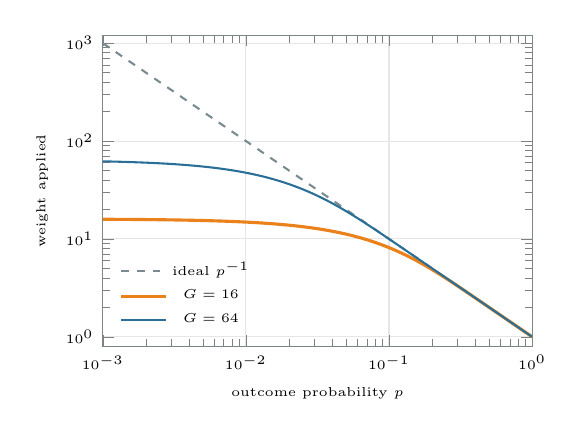
\begin{tikzpicture}[scale=0.94, transform shape]
\begin{axis}[
  width=5.8cm, height=4.2cm, scale only axis,
  xlabel={outcome probability $p$}, ylabel={weight applied},
  xmode=log, ymode=log,
  xmin=1e-3, xmax=1, ymin=0.8, ymax=1200,
  xtick={1e-3,1e-2,1e-1,1}, ytick={1,10,100,1000},
  label style={font=\tiny}, tick label style={font=\tiny},
  axis line style={mTeal!60}, grid=major, grid style={mTeal!12},
  legend style={font=\tiny, draw=none, fill=none, at={(0.02,0.03)}, anchor=south west},
]
  \addplot[mGrey, thick, dashed, domain=1e-3:1, samples=120]{1/x};
  \addlegendentry{ideal $p^{-1}$}
  \addplot[mOrange, very thick, domain=1e-3:1, samples=160]{(1-(1-x)^16)/x};
  \addlegendentry{$G=16$}
  \addplot[mBlue, thick, domain=1e-3:1, samples=160]{(1-(1-x)^64)/x};
  \addlegendentry{$G=64$}
\end{axis}
\end{tikzpicture}
\end{column}

\begin{column}{0.47\textwidth}
\footnotesize
\textbf{A finite group cannot apply an unbounded correction.}

\medskip
The ideal weight $p^{-\alpha}$ grows without limit as an outcome gets rarer. What
a group of $G$ can apply saturates, because a rare outcome is seen at most once,
at frequency $1/G$:
\[
  w_G(p)\;\longrightarrow\;\min\{G,1/\varepsilon\}^{\alpha}.
\]

\smallskip
Every part meets this ceiling from a different direction:

\smallskip
{\scriptsize
\begin{tabular}{@{}ll@{}}
Part 2 & finds it, and gets $\alpha_c$ for $K=2$ \\
Part 3 & shows $K>2$ needs a strictly larger $\alpha$ \\
Part 4 & verifies it over 19{,}125 points \\
Part 5 & shows only $\omega(1)/\omega(G)$ decides it \\
\end{tabular}}

\smallskip
At $\alpha=1$ the curve above is exactly $(1-(1-p)^G)/p$, proved in Part 5.
\end{column}
\end{columns}
\end{frame}

% --------------------------------------------------------------- O3
\begin{frame}{Conclusions and Limitations}

\begin{columns}[T,onlytextwidth]
\begin{column}{0.48\textwidth}
\footnotesize
\textbf{What a practitioner should take away}

\begin{itemize}\setlength\itemsep{3pt}
  \item Pick $G$ first. If $\min\{G,1/\varepsilon\}<r_{\max}/r_{\min}$, no
        exponent and no amount of training will keep the weak outcomes.
  \item Do not set $\varepsilon$ above $1/G$ without checking: it introduces a
        second, independent ceiling.
  \item For $K$ outcomes, the pairwise threshold is optimistic. At $G=16$ the
        weakest of five outcomes needs $\alpha=0.886$, not $0.580$.
  \item A moving average buys the variance of a $19\times$ larger group at
        $\beta=0.1$ with no extra rollouts, but it makes training ring if
        $\beta<4h\lambda$.
\end{itemize}
\end{column}

\begin{column}{0.48\textwidth}
\footnotesize
\textbf{What we are not claiming}

\begin{itemize}\setlength\itemsep{3pt}
  \item Everything is the outcome-selection bandit. Our update is
        group-REINFORCE without GRPO's advantage standardisation or PPO clipping,
        so the conclusions are about the \emph{weight rule}, not the whole
        algorithm.
  \item The $\alpha$-matched offset we derived is second order, not exact, and it
        costs dynamic range when $\alpha>1$.
  \item A per-outcome moving average assumes a small, enumerable outcome set.
        That is true here and false for the paper's LLM setting.
  \item The global convergence proof for general $\alpha$ is not attempted. We
        state the fixed point analytically and demonstrate convergence
        numerically from many initial conditions.
\end{itemize}
\end{column}
\end{columns}
\end{frame}

% --------------------------------------------------------------- closing
\begin{frame}[standout]
  Thank you\\[2mm]
  {\normalsize Questions}
\end{frame}

\end{document}
